\documentclass[tikz,border=10pt]{standalone}
\usetikzlibrary{shapes.geometric, calc}

\begin{document}
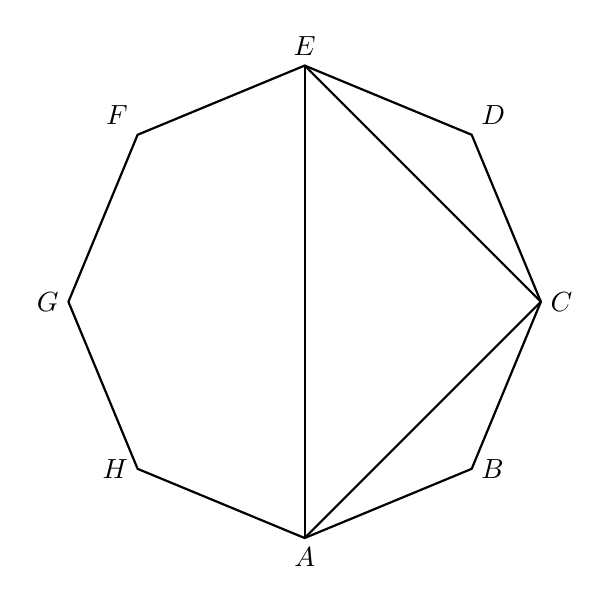
\begin{tikzpicture}[line cap=round, line join=round, >=stealth]

    % 1. 定义基本参数
    \def\radius{3} % 正八边形的外接圆半径
    \def\startangle{-90} % A点在最下方，即-90度

    % 2. 计算并标定正八边形的8个顶点 (A 到 H)
    % 360 / 8 = 45度每个步进
    \foreach \i [count=\n] in {0, 45, ..., 315} {
        \coordinate (V\n) at (\startangle+\i:\radius);
    }

    % 给顶点赋予题目中的字母名称
    % V1=A, V2=B, V3=C, V4=D, V5=E, V6=F, V7=G, V8=H
    \coordinate (A) at (V1);
    \coordinate (B) at (V2);
    \coordinate (C) at (V3);
    \coordinate (D) at (V4);
    \coordinate (E) at (V5);
    \coordinate (F) at (V6);
    \coordinate (G) at (V7);
    \coordinate (H) at (V8);

    % 3. 绘制正八边形的边界线
    \draw[thick] (A) -- (B) -- (C) -- (D) -- (E) -- (F) -- (G) -- (H) -- cycle;

    % 4. 绘制内部辅助连线 / 对角线
    \draw[thick] (A) -- (E); % 垂直中心线
    \draw[thick] (A) -- (C); % 连接A、C
    \draw[thick] (E) -- (C); % 连接E、C

    % 5. 标注顶点文字
    % 使用 anchor 或自动 position 调整标签位置，确保不被线条遮挡
    \node[below] at (A) {$A$};
    \node[right] at (B) {$B$};
    \node[right] at (C) {$C$};
    \node[above right] at (D) {$D$};
    \node[above] at (E) {$E$};
    \node[above left] at (F) {$F$};
    \node[left] at (G) {$G$};
    \node[left] at (H) {$H$};

\end{tikzpicture}
\end{document}